\RequirePackage[l2tabu, orthodox]{nag}
\documentclass[11pt,a4paper]{article}
%\usepackage[sc]{mathpazo}
\usepackage{termpaper}
%\usepackage{natbib}   
%\bibliographystyle{plainnat}
%\bibliographystyle{apalike}   % Or any other style you like
%\bibliographystyle{natbib} % kürzt automatisch vornamen ab und so zeug 

\usepackage[english]{babel}
\usepackage[hidelinks]{hyperref}
%\usepackage{hyperref}
\usepackage[T1]{fontenc}
\usepackage[utf8]{inputenc}
\usepackage{amsbsy,amsmath,amssymb,amsthm}
\usepackage{bbm}
\usepackage{bbold}
%\usepackage{bm}
\usepackage{braket}
\usepackage{caption}
\usepackage{color}
\usepackage{colortbl}
\usepackage{float}
\usepackage{framed}
\usepackage{graphicx}
\usepackage{ifthen}
\usepackage{listings}
%\usepackage{natbib}
\usepackage{scalefnt}
\usepackage{setspace}
\usepackage{textcomp}
\usepackage[dvipsnames]{xcolor}
\usepackage{tikz}
\usepackage{verbatim}

\usepackage{xifthen}
\usepackage{subcaption}
\usepackage[plain]{fancyref} % add page number to references (without plain)
\usepackage[kerning=true,tracking=true]{microtype} % better readability
\usepackage{todonotes}%\todo 
\usepackage{mathtools} % no idea 
\usepackage{nicefrac}%nicefrac allows typesetting fractions like 1/2. It is sometimes more readable than \frac.
\usepackage{paralist}%better itemize/enumerate
%\usepackage{savetrees} 
\usepackage{float} % use H to force float position



\usetikzlibrary{shapes,shapes.multipart,calc}

%\addto\captionsngerman{
%\renewcommand{\figurename}{Figure}%
%\renewcommand{\tablename}{Tab.}%
%}
\setlength{\parskip}{1.5ex plus0.5ex minus0.5ex}
\setlength{\parindent}{0em} 

%\sloppy \frenchspacing \raggedbottom 


%\usetikzlibrary{shapes,decorations,calc,arrows}
%\usetikzlibrary{external}
%\tikzexternalize[prefix=external]



% Prov makro
\DeclareMathOperator*{\Prov}{Prov}
\DeclareMathOperator*{\Var}{Var}


    \newcommand{\figref}[1]{\figurename~\ref{#1}}

\DeclareMathOperator*{\Proov}{Proof}
\newcommand{\NP}{\ensuremath{\mathcal{NP}}}
\newcommand{\TODO}[1][TODO]{\textcolor{red}{TODO}\todo{{#1}}}
\newcommand{\bigo}[1]{\ensuremath{\mathcal{O}(#1) }}


\newtheorem{theorem}{Theorem}
\newtheorem{definition}{Definition}
%\newtheorem{proof}{Proof}

%opening

\title{Polynomial Time Approximation Schemes for the Geometric Independent Set Problem}
\author{ \authorname{Abraham Hinteregger} \\
 \studentnumber{1025914} \\
 \curriculum{066931} \\
 \email{oerpli@outlook.com}
}
\setcounter{tocdepth}{3}
\begin{document}
% !TeX root = ./report.tex
\maketitle
%\listoftodos
\begin{abstract}
The geometric independent set problem is a special case of the independent set problem where the graph is the intersection graph of a set of geometric objects. The challenge of the geometric independent set problem is to find the biggest set of non-intersecting objects, i.e. the maximum independent set  (MIS). In this report I will present polynomial time approximation schemes (PTAS) for the geometric independent set problem for unit disk graphs (UDG) and for unit height rectangles. The geometric independent set problem is in general $\NP$- hard and therefore intractable. The algorithms presented here use different approaches to guarantee a polynomial running time for a constant approximation quality.
\end{abstract}

\tableofcontents



\section{Introduction}
The geometric independent set problem, i.e. finding a (maximum) set of non-intersecting geometric shapes is a problem that can arise in many different fields. In this report I will introduce algorithms to give approximate solutions for the MIS of unit disk graphs as well as for the geometric independent set problem for unit height rectangles. Unit disks may correspond to the area of influence of radio towers where frequencies can only be assigned to radio towers where this areas do not intersect (i.e. an independent set) to prevent interference~\cite{chamaret}. The maximum independent set of unit height rectangles could correspond to a labelling of a two dimensional map with a uniform font~\cite{agarwallabel}.
\subsection{Maximum independent set problem for graphs}
An independent set of a graph is a set of vertices that are not adjacent (connected with an edge). Finding a maximum independent set of an arbitrary graph is known to be an \NP-complete problem~\cite{misnp}. The best known exact algorithms have a runtime \bigo{1.22^n} \cite{exacta,exactb} (already quite good compared to the \bigo{n^2 2^n} naive brute force approach resulting from checking every subset of vertices).

If the graph is an interval intersection graph (see \Fref{sec:ig}) the MIS can be found in polynomial time (similar to the algorithm described in~\Fref{sec:greedyalg}) though for many (most) other intersection graphs it is still \NP-complete but approximate solutions can be found efficiently.


\subsection{Polynomial time approximation scheme}
As finding exact solutions for \NP-hard problems is not feasible in most cases, algorithms that solve a given instance of an intractable problem in polynomial time with a bounded loss in solution quality are of interest. A so called polynomial time approximation scheme (PTAS) is a family of algorithms that find a solution with a solution quality that is bounded by a factor of $(1+\varepsilon)$ for any $\varepsilon > 0$. %\todo{PTAS subsection überarbeiten, ist recht konfus aktuell}
%\begin{align*}
%\frac{S_{\text{OPT}}}{\rho} \quad \text{or}
%\quad \frac{S_{\text{OPT}}}{1\pm \varepsilon} \qquad (S_{\text{OPT}} \ldots \text{quality of optimal solution})

That is, if the optimal solution is $S_\text{OPT}$, the algorithm finds a solution with a quality of at least $\nicefrac{S_\text{OPT}}{1+\varepsilon}$ for a maximization problem and a solution with a quality of at most $(1+\varepsilon)S_\text{OPT}$ for a minimization problem.
%\end{align*} in polynomial time. For maximization problems $\rho> 1$, for minimization problems $\rho < 1$  (or $(1+\varepsilon)$ respectively $(1 - \varepsilon)$ for some $\varepsilon > 0$).
In both cases the algorithm has runtime polynomial in input-size though the dependency on $\varepsilon$ is usually not polynomial.

The subset of problems in \NP\ (actually $\mathcal{NPO}$ -- \NP-\ Optimization) with a polynomial time approximation scheme with constant quality bound (with \bigo{1}-approximation) is also called $\mathcal{APX}$. If the problem admits $1\pm \varepsilon$- approximation schemes (for arbitrarily small $\varepsilon > 0$) it is in the subset $\mathcal{PTAS}$ of $\mathcal{APX}$.
\subsection{Intersection graphs}\label{sec:ig}
An intersection graph of a set of objects represents how these objects intersect each other. \Fref{fig:igex} shows an example of such an arrangement and its corresponding intersection graph.
  \begin{figure*}[!h]
    \centering
    \begin{subfigure}[t]{0.5\textwidth}
        \centering

 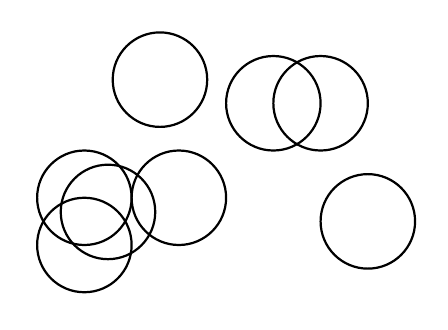
\begin{tikzpicture}[scale=0.6]
 \clip (-1.2,-1.2)rectangle(7.1,4.6);
 \newcommand{\centers}{(0,1),(0,0),(5,3),(2,1),(0.5,0.7),(4,3),(1.6,3.5),(6,0.5)}
 \foreach [count=\i] \coord in \centers{\draw[thick] \coord circle(1);}
 \end{tikzpicture}
      \caption{Geometric shapes (unit disks)}
\end{subfigure}%
  ~ 
 \begin{subfigure}[t]{0.5\textwidth}
      \centering
 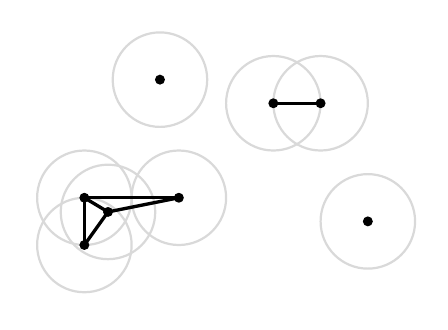
\begin{tikzpicture}[scale=0.6]
 \clip (-1.2,-1.2)rectangle(7.1,4.6);
    % link centers if circles intersect
      \newcommand{\centers}{(0,1),(0,0),(5,3),(2,1),(0.5,0.7),(4,3),(1.6,3.5),(6,0.5)}
      \foreach [count=\i] \coord in \centers{\draw[gray!30,thick] \coord circle(1);}  
        \foreach[count=\i] \a in \centers {
      \foreach[count=\j] \b in \centers {
        \ifnum \j < \i
          \draw[very thick] let \p1=\a, \p2=\b, \n1={veclen(\x1-\x2,\y1-\y2)} in
            {\ifdim \n1 < 2 cm \a -- \b \fi};
        \fi
      }
    }
    % draw circles
    \foreach \coord in \centers{\fill \coord circle(3pt);}
  \end{tikzpicture}
        \caption{Corresponding intersection graph}
    \end{subfigure}
    \caption{Arrangement of geometric shapes and corresponding intersection graph}\label{fig:igex}
\end{figure*}

It is also possible to reduce the edge set of the intersection graph to e.g.\ those edges where the corresponding objects intersect on an area bigger than a certain threshold (e.g. finding feasible locations for base stations where overlapping regions are inefficient). An example of this is in \Fref{fig:igex2} with a threshold of $20\%$ of the circle area.
\begin{figure}\centering


\end{figure}

  \begin{figure*}[!h]
    \centering
    \begin{subfigure}[t]{0.5\textwidth}
        \centering

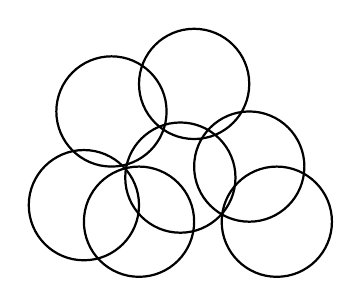
\begin{tikzpicture}[scale=0.35,rotate=90]
\newcommand{\centers}{(0,0),(2,1),(1.6,3.5),(0,5),(5,3),(0.6,7),(4,6)}
{ \foreach \coord in \centers{\draw[thick] \coord circle(2);}}        
\newcommand{\centerss}{(0,0),(1.6,3.5),(5,3),(0.6,7),(4,6)}
\end{tikzpicture}
   \caption{Geometric shapes (unit disks)}
\end{subfigure}%
  ~ 
 \begin{subfigure}[t]{0.5\textwidth}
      \centering
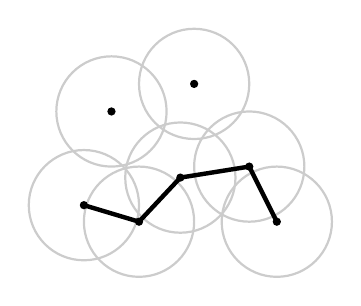
\begin{tikzpicture}[scale=0.35,rotate=90]
\newcommand{\centers}{(0,0),(2,1),(1.6,3.5),(0,5),(5,3),(0.6,7),(4,6)}
{ \foreach \coord in \centers{\draw[gray!40, thick] \coord circle(2);}}        
{\draw[ultra thick] (0,0) -- (2,1) -- (1.6,3.5) -- (0,5)-- (0.6,7);}
{ \foreach \coord in \centers{\fill \coord circle(0.15);}}        
\end{tikzpicture}
      \caption{Corresponding intersection graph}
    \end{subfigure}
    \caption{Edges in IG correspond to at least $20\%$ intersecting area of the circles.}\label{fig:igex2}
\end{figure*}


\subsubsection{Construction of intersection graphs from geometric objects}
Given an arrangement $\mathcal A$ of $n$ geometric objects its intersection graph $G=(V,E)$ can be obtained in the following way: 
\begin{itemize}
\item The vertex set $V$ consists of $n$ vertices --- each of them uniquely represents one of the geometric shapes of $\mathcal A$
\item For every pair $s_i, s_j$ of vertices check whether they intersect each other and add the edge $\langle i, j\rangle$ to the edge set $E$ if this is the case. 
\end{itemize}
Obviously the runtime of this scheme is \bigo{n^2}. The worst case performance of finding an intersection graph is always \bigo{n^2} as there can be a quadratic amount of intersections (if all objects intersect each other). If there are less intersection this can usually be improved to \bigo{n \log n + I} where $I$ is the amount of intersections (once again, with quadratic upper bound) and the other term is from sorting the objects according to some criterion, e.g. the leftmost point of the object on the x-axis. Sweepline algorithms are used for this, the best known is the Bentley--Ottman algorithm for line segments~\cite{bentleyott} with runtime \bigo{n \log n +n I}. 

\subsubsection{Geometric representation of  intersection graph}
%Every graph can be interpreted as intersection graph (Erdös et al.~\cite{erdos1966representation} gave a constructive proof with  of some weirdly shaped geometric objects\todo{genauer erklären},
Finding a valid representation, i.e. a mapping  $f : V \to \mathbb R^d$, from the set of vertices to a vector representation of the geometric objects defined by $x_1, \ldots x_d \in \mathbb R$ (e.g. for disks in the plane $d=3$ ($x-,y-$ coordinates and radius), for rectangles $d=4$ (two points with two coordinates each)) is in many cases a $\NP$-hard problem \cite{nphard} and it is therefore not feasible to find a geometric representation of a given graph and use the additional information to simplify the general independent set problem.

\subsection{Robust algorithms}
An algorithm $\mathcal A$ computes a function $f: \mathcal G \to \mathcal H$. If the algorithm is only able to compute the correct result $f(i)$ for $i \in \mathcal U \subset G$ there are elements in $\mathcal G$ that are not in $\mathcal U$ and therefore the algorithm may not compute the correct result (or may not terminate at all).
\begin{definition}
 An algorithm $\mathcal A$ computes $f$ \textit{robustly on $\mathcal U$} if:
\begin{itemize}
\item for all instances $i\in\mathcal U$ it returns the correct result $f(i)$
\item for all instances $i\in\mathcal G\setminus \mathcal U$ the algorithm either returns $f(i)$ or a certificate showing that $i\notin \mathcal U$.
\end{itemize}
\end{definition}

\section{M(W)IS for unit disk graphs (UDG)}
In this section I will present a robust PTAS for both, the weighted and unweighted unit disk graph independent set problem as introduced by Nieberg et al.~\cite{nieberg}. The algorithm does not depend on the geometric representation, though the polynomial runtime is only guaranteed if such a representation exists because it uses the area $\pi$ of the unit disks to get an upper bound on the amount of disks in an independent set of a certain area.
\subsection{Preliminaries}
A unit disk graph $G=(V,E)$ is a graph where there exists a geometric representation $f:V \to \mathbb R^2$ i.e.\ a function that maps every vertex to a point to the center point on the real Cartesian plane of the disk in the geometric representation such that:
\begin{align}
(u,v) \in E \leftrightarrow ||f(u) - f(v)|| \leq 2.\label{eq:maxdist}
\end{align}
As finding this representation is \NP-hard it is not feasible to compute a valid representation of the given graph. Furthermore it is also \NP-hard to determine if a valid geometric representation even exists~\cite{nphard}.

Furthermore, let $\rho = 1+\varepsilon$ denote the desired approximation ratio where $\varepsilon > 0$. 
\subsection{MIS for unweighted UDG}\label{sec:misudg}
The algorithm is given a UDG $G = (V,E)$ and the desired result is a set $I \subseteq V$ that has a cardinality that is at least $\alpha(G)\rho^{-1}$ where $\alpha(G)$ is the maximum size of an independent set in $G$.
The algorithm starts at an arbitrary node $v\in V$ and computes the sets
\begin{align*}
N_r = N_r(v) := \{w\in V|w \text{ has distance at most $r$ from $v$}\}
\end{align*} for $r = 0,1,\ldots$. Starting from $N_0$ the algorithm computes the maximum independent set $I_r \subset N_r$ of these $r$-neighborhoods until the condition
\begin{align}
|I_{r+1}| > \rho|I_r| \label{eq:udgcond}
\end{align}is no longer fulfilled - let $\bar r$ be the smallest $r$ where \fref{eq:udgcond} is violated. Such a $\bar r$ must exist and it has a constant upper bound.
\Fref{fig:udgalg} shows how these neighborhoods are selected on an example graph.
% !TeX root = ../report.tex

\DeclareRobustCommand{\circN}[1]{\tikz[anchor=base,baseline=-.125cm]{\node(n){};\fill (n) circle(0.15);}}
\DeclareRobustCommand{\circI}[1]{\tikz[anchor=base,baseline=-.125cm]{\node(n){};\fill (n) circle(0.15);\draw[ultra thick, MidnightBlue](n)circle(0.25);}}
\DeclareRobustCommand{\circX}[1]{\tikz[anchor=base,baseline=-.125cm]{\node(n){};\fill[gray] (n) circle(0.1);}}

\begin{figure}[t]
\centering
\newcommand{\vv}{v_0}
    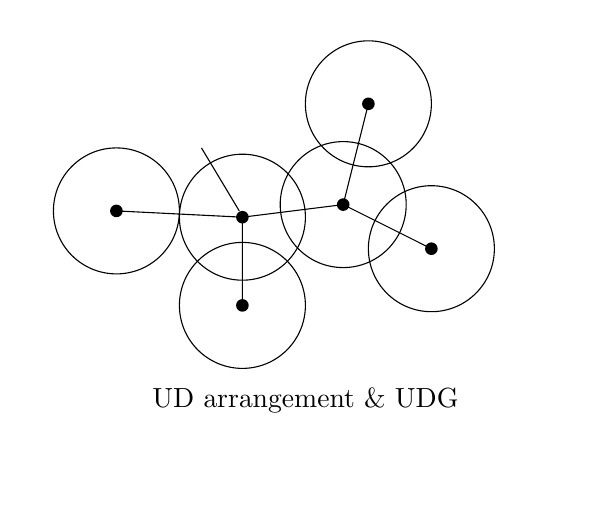
\begin{tikzpicture}[scale=0.8]
    \
    \coordinate (V) at (2,2);
    \coordinate (V2) at (3.6,2.2);
   \newcommand{\None}{(2,0.6),(0,2.1),(V2)}
   \newcommand{\Ntwo}{(5,1.5),(4,3.8)}

   {  
   	\fill (V) circle(0.1);
	\foreach \coord in \None{\fill \coord circle(0.1);}
	\foreach \coord in \Ntwo{\fill \coord circle(0.1);}
	\foreach \coord in \None{\draw (V) --\coord;}
	\foreach \coord in \Ntwo{\draw (V2) --\coord;}
	
}        
   {
	 \draw (V) circle(1);
   	 \foreach \coord in \None{\draw \coord circle(1);}
	\foreach \coord in \Ntwo{\draw \coord circle(1);}
}        
{\draw[] ($(V)+(-0.05,0.1)$)--+(-0.6,1)node[above]{$\vv$};}       
\coordinate(CAP) at (3,1);
\node [below=1.25cm, align=flush center,text width=5cm] at (CAP){UD arrangement \& UDG};
\draw[white] (-1.4,5) rectangle(7.2,-2.5);\end{tikzpicture}
%%%%%
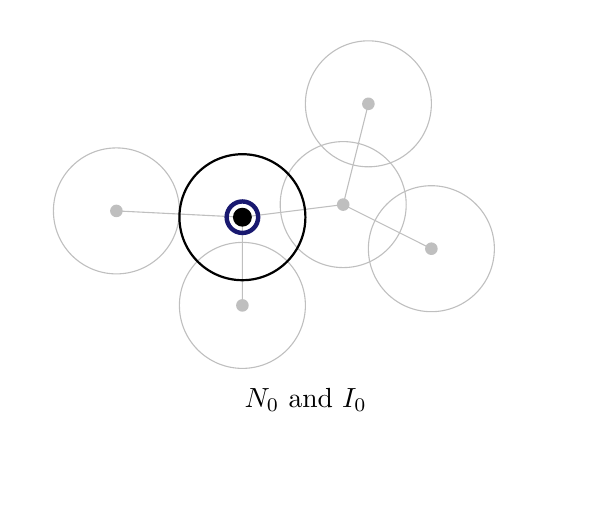
\begin{tikzpicture}[scale=0.8]
    \coordinate (V) at (2,2);
    \coordinate (V2) at (3.6,2.2);
   \newcommand{\None}{(2,0.6),(0,2.1),(V2)}
   \newcommand{\Ntwo}{(5,1.5),(4,3.8)}

      
   {

	\foreach \coord in \None{\fill[gray!50] \coord circle(0.1);}
	\foreach \coord in \Ntwo{\fill[gray!50] \coord circle(0.1);}
	\foreach \coord in \None{\draw[gray!50] (V) --\coord;}
	\foreach \coord in \Ntwo{\draw[gray!50] (V2) --\coord;}
   	 \foreach \coord in \None{\draw[gray!50] \coord circle(1);}
	\foreach \coord in \Ntwo{\draw[gray!50] \coord circle(1);}
     	\fill[] (V) circle(0.15);
     	\draw[thick] (V) circle(1);	
}   

   {  


\draw[ultra thick,MidnightBlue] (V) circle(0.25);
}  

\coordinate(CAP) at (3,1);
 \node [below=1.25cm, align=flush center,text width=5cm] at (CAP){$N_0$ and $I_0$};
\draw[white] (-1.4,5) rectangle(7.2,-2.5);\end{tikzpicture}
\\
%%%
%%%%%
    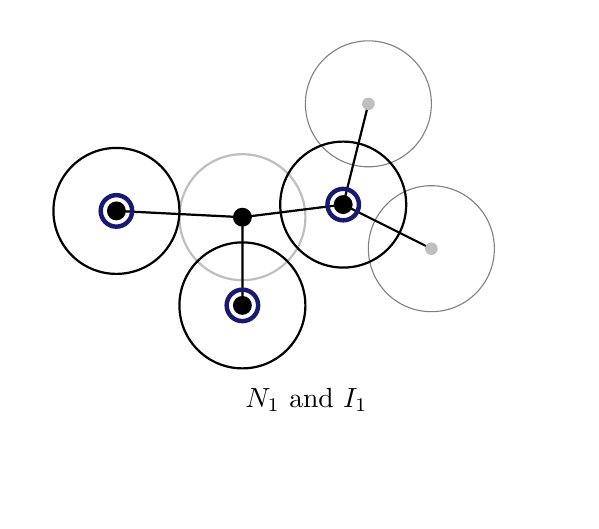
\begin{tikzpicture}[scale=0.8]
    \
\coordinate (V) at (2,2);
\coordinate (V2) at (3.6,2.2);
\newcommand{\None}{(2,0.6),(0,2.1),(V2)}
\newcommand{\Ntwo}{(5,1.5),(4,3.8)}
%\draw[thick] (V) circle(1);
\draw[thick,gray!50] (V) circle(1);       
\foreach \coord in \Ntwo{\draw[gray] \coord circle(1);}
\foreach \coord in \None{\draw[thick] \coord circle(1);}
\foreach \coord in \Ntwo{\draw[gray] (V2) --\coord;}
\foreach \coord in \None{\draw (V) --\coord;}
\fill (V) circle(0.15);
    
\foreach \coord in \Ntwo{\draw[thick] (V2) --\coord;}
\foreach \coord in \None{\draw[thick] (V) --\coord;}
\foreach \coord in \None{\draw[ultra thick,MidnightBlue] \coord circle(0.25);}
\foreach \coord in \None{\fill[] \coord circle(0.15);}
\foreach \coord in \Ntwo{\fill[gray!50] \coord circle(0.1);}

\coordinate(CAP) at (3,1);
\node [below=1.25cm, align=flush center,text width=5cm] at (CAP){$N_1$ and $I_1$}; 
\draw[white] (-1.4,5) rectangle(7.2,-2.5);\end{tikzpicture}
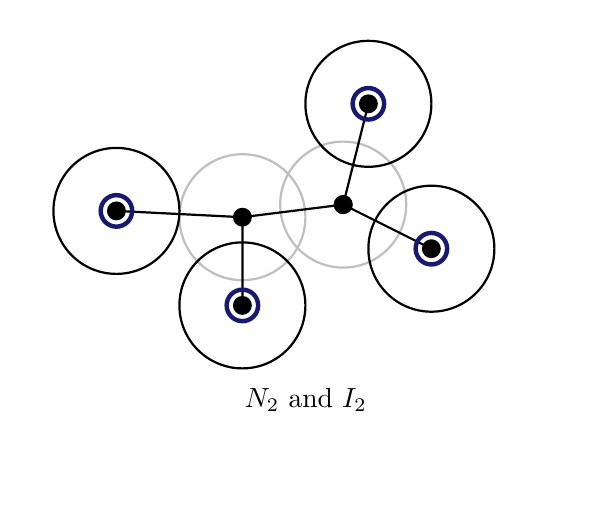
\begin{tikzpicture}[scale=0.8] % i guess this is the bist picture of them all. use this for copypasting later
\coordinate (V) at (2,2);
\coordinate (V2) at (3.6,2.2);
\newcommand{\None}{(2,0.6),(0,2.1),(V2)}
\newcommand{\Nonee}{(2,0.6),(0,2.1)}
\newcommand{\Ntwo}{(5,1.5),(4,3.8)}

%\draw[thick] (V) circle(1);
%\draw[thick] (V2) circle(1);
\foreach \coord in \Ntwo{\fill \coord circle(0.15);}
\foreach \coord in \None{\fill \coord circle(0.15);}
\draw[thick,gray!50] (V) circle(1);
\draw[thick,gray!50] (V2) circle(1);
\foreach \coord in \Nonee{\draw[thick] \coord circle(1);}
\foreach \coord in \Ntwo{\draw[thick] \coord circle(1);}
\foreach \coord in \Ntwo{\draw[thick] (V2) --\coord;}
\foreach \coord in \None{\draw[thick] (V) --\coord;}
\foreach \coord in \Nonee{\draw[ultra thick,MidnightBlue] \coord circle(0.25);}
\foreach \coord in \Ntwo{\draw[ultra thick,MidnightBlue] \coord circle(0.25);}
\fill (V) circle(0.15);
\fill (V2) circle(0.15);
%\fill[gray] (V) circle(0.15);
%\fill[gray] (V2) circle(0.15);
\coordinate(CAP) at (3,1);
\node[below=1.25cm, align=flush center,text width=5cm] at (CAP){$N_2$ and $I_2$};
\draw[white] (-1.4,5) rectangle(7.2,-2.5);
\end{tikzpicture}
\caption{Unit disk graph (with disk representation) and the sets calculated by the algorithm. Nodes in a neighborhood set $N_r$ are marked with \circN\ \ and nodes in independent sets $I_r$ are marked with \circI \ . Not yet considered nodes are marked with \circX\ \ .  The algorithm starts at $\vv$ and takes neighborhoods $N_r$ of increasing size $r$ until the size of the independent set $I_r\subset N_r$ is below a certain threshold.}\label{fig:udgalg}
\end{figure}

\begin{theorem}[Nieberg et al.~\cite{nieberg}]
There exists a constant $c= c(\rho)$ such that $\bar r \leq c$
\end{theorem}
\begin{proof}
Due to \Fref{eq:maxdist} any vertex $w\in N_r$  satisfies
\begin{align*}
||f(w) - f(v)|| \leq 2r. 
\end{align*}
it is therefore possible to draw a circle with radius $R = 2r+1$ that contains all disks representing the vertices in $N_r$. This circle also contains the disk representations of the vertices in $I_r$ which have a disjoint area of $\pi$ each (as their radius equals $1$). This leads to an upper bound on the size of each independent set:
\begin{align}
|I_r| \leq \pi R^2 /\pi = (2r+1)^2 = O(r^2).\label{eq:udupper}
\end{align}
From \Fref{eq:udgcond}follows:
\begin{align}
|I_r| > \rho|I_{r-1}| > \ldots  > \rho^r|I_0| = \rho^r.\label{eq:udglower}
\end{align}
Combining \eqref{eq:udupper} and \eqref{eq:udglower} yields
\begin{align}
\rho^r < |I_r| \leq O(r^2), \label{eq:upperboundlol}
\end{align}
an inequality (two of them actually) where the lower bound grows asymptotically faster then the upper bound with increasing $r$ -- therefore there exists a constant upper bound $c(\rho)$ for $r$.
\end{proof}
The fact that the size of the independent sets calculated for the various $N_r$ ($r\leq \bar r$) implies a polynomial runtime of $\bigo{n^{C^2}}$ (where $C = \bigo{r} = \bigo{1/\varepsilon^2 \log (1/\varepsilon}$).
The full algorithm proceeds as follows:
\begin{enumerate}
\item Calculate the independent set $I_{\bar r}$ starting from an arbitrary vertex $v$.
\item Remove the vertices in $N_{\bar r +1 }$ from the graph $G$ to get the graph $G' = (V',E') = G\setminus N_{\bar r +1}$ (including edges incident to any of the removed vertices).
\item Repeat the previous two steps for $G'$ until there is no vertex left i.e.\ $G' = (\varnothing,\varnothing)$.
\item Combine all $I_{\bar r}$ to get a $\rho$-approximate maximum independent set.
\end{enumerate}




\subsubsection{Proof of correctness \& approximation guarantee}

The correctness and approximation guarantee follows from the following two theorems by Nieberg et al.~\cite{nieberg}:
\begin{theorem}
Suppose that we can compute an independent set $I'\subset V\setminus N_{\bar r+1}$ of the graph $G'$. Then $I:=I_{\bar r} \cup I'$ is an independent set for $G$.
\end{theorem}
\begin{proof}
A vertex $v\in I'\subset V'$ has no neighbor $n\in N_{\bar r}$ as the distance between $v$ and any such $n$ is at least $\bar r +2$ (else it would have been in $N_{\bar r}$ and removed from the vertex set of $G'$). Therefore $I$ is an independent set. 
\end{proof}

\begin{theorem}
Suppose inductively that we can compute a $\rho$-approximate independent set $I'\subset V\setminus N_{\bar r+1}$ of the graph $G'$. Then $I:=I_{\bar r} \cup I'$ is a  $\rho$-approximate independent set for $G$.
\end{theorem}
\begin{proof}
As $\bar r$ is chosen in such a way that the maximum independent set of $N_{\bar r}$ is a $\rho$-approximate independent set of $N_{\bar r +1}$  (ensured by \Fref{eq:udgcond}):
\begin{align*}
|I_{\bar r +1}| \leq \rho|I_{\bar r}|.
\end{align*}
Therefore the following holds:
\begin{align*}
\alpha(G[N_{\bar r +1}]) \leq \rho|I_{\bar r}|  = \rho\alpha(N_{\bar r}).
\end{align*}
Furthermore it is obvious that the size of an independent set of a graph is at most as large as the sum of the sizes of independent sets of subgraphs that form a partition of the initial graph. Applying this here yields
\begin{align*}
\alpha(G)& \leq \alpha(G[N_{\bar r +1 }]) + \alpha(V\setminus G[N_{\bar r +1}]) \leq \rho|I|\\
\alpha(G)& \leq  \rho|I|,
\end{align*} and thus proves that the desired approximation guarantee is fulfilled.
%\TODO[maybe make this proof a little easier to understand]
\end{proof}
\subsection{MWIS for weighted UDG}\label{sec:mwisudg}
If the given UDG has a vector $\vec w$ assigning positive values $w_i$ to every vertex $v_i$ and the objective is to find an independent set of maximum weight the algorithm described in \Fref{sec:misudg} can be easily adapted to yield an independent set that has a weight that is at least $\rho^{-1}$ the weight of the independent set with the maximum weight.
The following things have to be adapted:
\paragraph{Starting node $v_0$:} Don't start at an arbitrary node $v_0$ but at the node with the heighest weight.
\paragraph{Stopping criterion:} Modify the stopping criterion in \Fref{eq:udgcond} to consider the weight instead of only the size. The function $W: V^n\to \mathbb R$ maps vertices to their weight and sets of vertices to the sum of their weight. 
\begin{align*}
W(I_{r+1}) > \rho W(I_r)
\end{align*}
Obtaining the bound to get a constant upper bound (as in \Fref{eq:upperboundlol}) is rather straightforward:\\
\begin{theorem}[Nieberg et al.~\cite{nieberg}]
There exists a constant $c= c(\rho)$ such that $\bar r \leq c$
\end{theorem}
\begin{proof}
The idea of the proof is the same as for the unweighted case. As the upper bound use:
\begin{align*}
W(I_r) &= \sum_{i\in I_r}W(v_i)\leq \sum_{i\in I_r}W(v_0) = |I_r|w_0
\intertext{where $w_0$ is the weight of $v_0$ -- the vertex with highest weight. And the lower bound use:}
W(I_r) &> \rho W(I_{r-1} > \ldots > \rho^r W(I_0) = \rho^r  w_0
\end{align*}As it still holds that $I_r$ is bounded by $\bigo{r^2}$ (using the area of the unit disks) we get the same upper and lower bounds but with an additional constant factor for the weight of the initial node. 
\end{proof}

\subsection{Robustness}
The algorithms outlined in \Fref{sec:misudg} and \Fref{sec:mwisudg} are PTAS with the desired solution quality as long as the graph really is a unit disk graph. To get a robust PTAS for arbitrary graphs from this there are some minor modifications necessary. Observe, that in both cases the approximation quality as well as the overall correctness did not depend on any properties of a UDG. Only for getting the constant bound on the sizes of the independent sets $I_r$ the area of the disks was used. \\
The only necessary modification is therefore to look whether an independent set of size $|I_r^*| > (2r+1)^2$ can be found and if this is the case return it as certificate that the given graph is not a UDG. Finding this set is also possible in polynomial time as not the maximum independent set $I_r\subset N_r$ has to be found (the maximum size of this independent set would be unbounded and therefore impossible to determine in polynomial time) but only an independent subset with a size of at least $(2r+1)^2+1$ is necessary which is still possible in polynomial time.

\section{MIS for unit height rectangles}
The maximum independent set problem for unit height rectangle is a problem that arises when labelling maps. The goal is to find a maximum non-intersecting set of possible labels in the plane to ensure legibility. In this section I will present a $2$-approximation algorithm  with \bigo{n \log n} runtime for the unweighted MIS problem for unit height rectangles introduced by Agarwal et al.~\cite{agarwallabel} which can be improved upon with a dynamic programming approach to get a $(1+\nicefrac{1}{k})$-approximation algorithm with runtime \bigo{n \log n + n^{2k-1}} for $k\geq 1$. The idea of the improvement will be presented here, for the technical details the original paper has to be consulted. For this algorithms the arrangement of rectangles is required.
\subsection{A $2$-approximation algorithm}
The set of $n$ rectangles $R$ with unit height is given. The maximum independent set of rectangles is $I_\text{OPT}$. To get a $2$-approximate independent set, the algorithm partitions the $n$ rectangles into disjunct subsets, calculates the maximum independent set of those subsets and returns the conjunction of those independent sets. To divide the rectangles into sets horizontal lines $\ell_1, \ell_2,\ldots,\ell_m$ where $m\leq n$ are drawn such that the following three conditions hold:
\begin{itemize}
\item The distance between two adjacent lines is $>1$. i.e.\ bigger than the height of a rectangle
\item Each line intersects at least one rectangle
\item Each rectangle is intersected by exactly one line
\end{itemize}
To find the correct positions for the lines, first sort the rectangles according to their vertical coordinates and draw the first line at the top of the rectangle with smallest $y$-coordinate and the following lines at the top of the rectangle with the smallest $y$-coordinate that is not yet intersected by a line.  \Fref{fig:uhr1a} illustrates this. Now every rectangle has an intersecting line and the initial arrangement of rectangles is partitioned into sets $R_1,\ldots,R_m$ where for every $1\leq i \leq m$ the set $R_i$ contains those rectangles that are intersected by the line $\ell_i$.

Due to the fact that the distance between two lines is bigger than the height of the rectangles a rectangle in the set $R_i$ can only intersect with rectangles in the sets $R_i$ and $R_i\pm1$. Therefore the independent sets $I_i$ of the even sets $R_{2n}$ and the odd sets $R_{2n+1}$ ($0\geq n \geq \nicefrac{m}{2}$) can be combined to two independent sets $I_{\text{odd}} = \bigcup_{n> 0} I_{2n}$ and $I_{\text{even}} = \bigcup_{n\geq 0} I_{2n+1}$.

\subsubsection{Greedy algorithm for MIS of intervals}\label{sec:greedyalg}
The MIS of every subset $R_i$ can be found in polynomial time with a greedy algorithm. As can be seen in \Fref{fig:uhr1c} two rectangles that are intersected by a common horizontal line only intersect each other iff the intervals of their $x$-coordinates intersect each other. Therefore the problem of finding a MIS of the rectangles in one of the sets $R_i$ can be reduced to finding a MIS of the horizontal projection of these rectangles. For this a greedy algorithm with runtime \bigo{n\log n} exists. The idea of this algorithm is the following inductive argument: For every point $p$ on the $x$-axis at most one interval in the MIS can be \textit{active}, i.e.\ having a start point $s$ and an end point $e$ s.t.\ $s\leq p\leq e$. It follows that if two (or more) intervals intersect each other at one point at most one of these intervals can be added to an independent set. Choosing the interval with the lowest endpoint allows choosing more intervals after this interval (see \Fref{fig:uhr1d}). 

\begin{figure*}[!h]
\centering
\begin{subfigure}[t]{0.5\textwidth}
\centering
\definecolor{cadmiumred}{rgb}{0.89, 0.0, 0.13}
\definecolor{cadmiumgreen}{rgb}{0.01, 0.75, 0.24}
\begin{tikzpicture}
\draw[very thick,cadmiumred] (1,0) rectangle+(1,1);
\draw[very thick,cadmiumred] (6,0) rectangle+(0.5,1);
\draw[very thick,cadmiumred] (3.5,0.2) rectangle+(1.5,1);
\draw[very thick,cadmiumred] (5.2,0.4) rectangle+(1,1);
\draw[very thick,cadmiumred] (3,0.8) rectangle+(0.9,1);

\draw[very thick,MidnightBlue] (2.2,1.3) rectangle+(1.5,1);
\draw[very thick,MidnightBlue] (1,1.4) rectangle+(1.9,1);
\draw[very thick,MidnightBlue] (3.5,1.6) rectangle+(2,1);

%\definecolor{darkpastelgreen}{rgb}
\draw[very thick,cadmiumgreen] (0.2,2.5) rectangle+(1.9,1);
\draw[very thick,cadmiumgreen] (6,2.5) rectangle+(1.2,1);
\draw[very thick,cadmiumgreen] (2.2,2.8) rectangle+(1.3,1);
\draw[very thick,cadmiumgreen] (1,2.9) rectangle+(0.7,1);
\draw[very thick,cadmiumgreen] (5.3,2.9) rectangle+(0.8,1);
\draw[very thick,cadmiumgreen] (3,3) rectangle+(1.5,1);
\draw[very thick,cadmiumgreen] (3.6,3.1) rectangle+(1,1);
\draw[very thick,cadmiumgreen] (4.7,3.3) rectangle+(0.5,1);

\draw[very thick,dashed] (0,1.0)--+(7.5,0) node[right] {$\ell_1$};
\draw[very thick,dashed] (0,2.3)--+(7.5,0)node[right] {$\ell_2$};
\draw[very thick,dashed] (0,3.5)--+(7.5,0)node[right] {$\ell_3$};
\end{tikzpicture}
\caption{Unit height rectangles partitioned into three sets $\color{cadmiumred}{R_1},\color{MidnightBlue}{R_2},\color{cadmiumgreen}{R_3}$ with intersecting lines $\ell_1,\ell_2,\ell_3$.}\label{fig:uhr1a}
\end{subfigure}%
  ~ \vline ~ 
 \begin{subfigure}[t]{0.5\textwidth}
      \centering
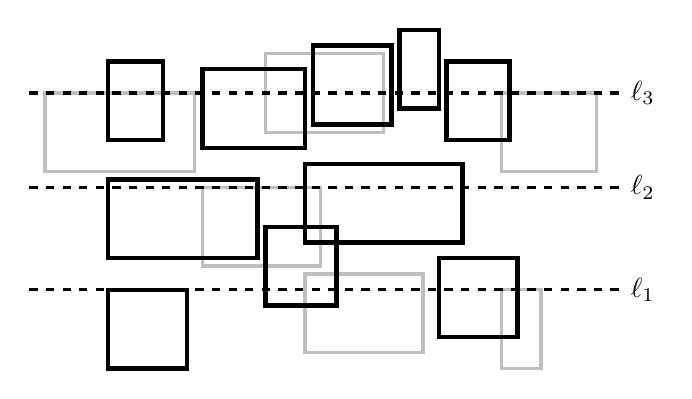
\begin{tikzpicture}[scale=1]
\draw[very thick,gray!50] (3.5,0.2) rectangle+(1.5,1);
\draw[very thick,gray!50] (6,0) rectangle+(0.5,1);

\draw[very thick,gray!50] (2.2,1.3) rectangle+(1.5,1);



\draw[ultra thick] (1,0) rectangle+(1,1);
\draw[ultra thick] (3,0.8) rectangle+(0.9,1);
\draw[ultra thick] (5.2,0.4) rectangle+(1,1);

\draw[ultra thick] (1,1.4) rectangle+(1.9,1);
\draw[ultra thick] (3.5,1.6) rectangle+(2,1);



\draw[very thick,gray!50] (3,3) rectangle+(1.5,1);
\draw[very thick,gray!50] (6,2.5) rectangle+(1.2,1);
\draw[very thick,gray!50] (0.2,2.5) rectangle+(1.9,1);
\draw[ultra thick] (1,2.9) rectangle+(0.7,1);
\draw[ultra thick] (2.2,2.8) rectangle+(1.3,1);
\draw[ultra thick] (3.6,3.1) rectangle+(1,1);
\draw[ultra thick] (4.7,3.3) rectangle+(0.5,1);
\draw[ultra thick] (5.3,2.9) rectangle+(0.8,1);


\draw[very thick,dashed] (0,1.0)--+(7.5,0) node[right] {$\ell_1$};
\draw[very thick,dashed] (0,2.3)--+(7.5,0)node[right] {$\ell_2$};
\draw[very thick,dashed] (0,3.5)--+(7.5,0)node[right] {$\ell_3$};
\end{tikzpicture}
\caption{MIS $I_1,I_2,I_3$ (black) for the sets $R_i$. Note that rectangles from IS of two adjacent sets ($I_i, I_{i\pm 1}$) may intersect each other.}
\end{subfigure}\\
 \begin{subfigure}[t]{0.5\textwidth}
\centering
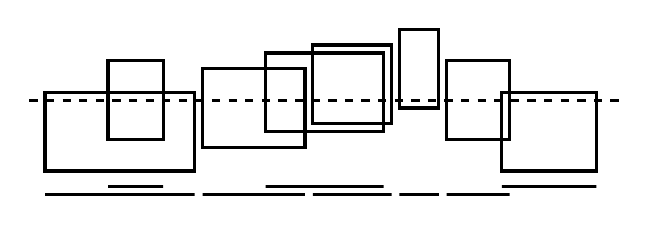
\begin{tikzpicture}[scale=1]
\draw[very thick] (1,2.9) rectangle+(0.7,1);
\draw[very thick] (3,3) rectangle+(1.5,1);
\draw[very thick] (6,2.5) rectangle+(1.2,1);
\draw[very thick] (0.2,2.5) rectangle+(1.9,1);
\draw[very thick] (2.2,2.8) rectangle+(1.3,1);
\draw[very thick] (3.6,3.1) rectangle+(1,1);
\draw[very thick] (4.7,3.3) rectangle+(0.5,1);
\draw[very thick] (5.3,2.9) rectangle+(0.8,1);
\draw[very thick,dashed] (0,3.4)--+(7.5,0);
\begin{scope}[yshift=2.2cm]
\draw[very thick] (0.2,0) rectangle+(1.9,0);
\draw[very thick] (1,0.1) rectangle+(0.7,0);
\draw[very thick] (2.2,0) rectangle+(1.3,0);
\draw[very thick] (3,0.1) rectangle+(1.5,0);
\draw[very thick] (3.6,0.0) rectangle+(1,0);
\draw[very thick] (4.7,0.0) rectangle+(0.5,0);
\draw[very thick] (5.3,0.0) rectangle+(0.8,0);
\draw[very thick] (6,0.1) rectangle+(1.2,0);
%\draw[very thick,dashed] (0,1)--+(7.5,0);
\end{scope}
\end{tikzpicture}
\caption{To find a MIS of $R_3$ only the $x$-coordinates have to be considered. Two rectangles intersect iff their projection to a horizontal line (below) intersects.}
\label{fig:uhr1c}
\end{subfigure}%
  ~ \vline ~ 
 \begin{subfigure}[t]{0.5\textwidth}
\centering
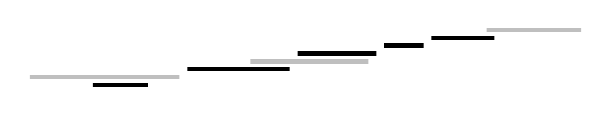
\begin{tikzpicture}[scale=1]
\draw[ultra thick] (1,0) rectangle+(0.7,0);
\draw[ultra thick,gray!50] (0.2,0.1) rectangle+(1.9,0);
\draw[ultra thick] (2.2,0.2) rectangle+(1.3,0);
\draw[ultra thick,gray!50] (3,0.3) rectangle+(1.5,0);
\draw[ultra thick] (3.6,0.4) rectangle+(1,0);
\draw[ultra thick] (4.7,0.5) rectangle+(0.5,0);
\draw[ultra thick] (5.3,0.6) rectangle+(0.8,0);
\draw[ultra thick,gray!50] (6,0.7) rectangle+(1.2,0);
%\draw[very thick,dashed] (0,1)--+(7.5,0);
\end{tikzpicture}
\caption{Horizontal projection of rectangles in $R_3$ ordered (in vertical direction) by their endpoint. Greedy algorithm adds interval with nearest endpoint (bottom to top in this figure) that does not intersect rectangles already in the set.}
\label{fig:uhr1d}
\end{subfigure}

    \caption{Illustration of the $2$-approximation algorithm for the unit height rectangle MIS problem.}\label{fig:uhr1}
\end{figure*}


\subsubsection{Correctness and proof of approximation quality}
\begin{theorem}
The set $I_{\text{even}} = \bigcup_{n> 0} I_{2n}$ obtained by combining the maximum independent sets $I_{n}$ of the sets $R_{n}$ for even $n$ is also a maximum independent set of $R_{\text{even}} = \bigcup_{n>0}R_{2n}$.
\end{theorem}
\begin{proof}
 The rectangles in this set are independent because a rectangle $r$ from the set $I_x\subseteq R_x$ can't intersect any other rectangle in the set $I_x$ because if this were the case $I_x$ would not be an independent set. Furthermore the rectangle $r$ can't intersect any rectangle $r'\in I_\text{even}\setminus I_x$ as $r$ and $r'$ both are intersected by a horizontal line with a vertical distance $2+\varepsilon$ with $\varepsilon>0$ and therefore the vertical distance between $r$ and $r'$ is at least $\varepsilon$. As every independent set $I_x$ is the MIS of $R_x$ the combination $I_\text{even}$ is also the MIS of $R_\text{even}$. The same arguments apply to the set $I_\text{odd}\subseteq R_\text{odd}$.\\
\end{proof}
The approximation quality guarantee follows from the fact that the MIS $I_\text{OPT}$ of all the rectangles is at most $I_\text{even} + I_\text{odd}$. Therefore choosing the bigger of the sets $I_\text{even}$ and $I_\text{odd}$ leads to a $2$-approximation in the case that $|I_\text{even}| = |I_\text{odd}|$. If one of the sets has more elements than the other the approximation is even better. 
\subsubsection{Runtime of $2$-approximation algorithm}
The runtime of the algorithm is dominated by the sorting of the rectangles which takes time \bigo{n \log n}. Partitioning the sorted rectangles with horizontal lines can be done in \bigo{n} by iteratively taking the first (i.e.\ having the smallest $y$-coordinate) not-yet-intersected rectangle and adding a line at it's upper $y$-coordinate. Finding the MIS of every set $R_i$ is also bounded by \bigo{n\log n} resulting from the sorting the rectangles in each of the sets of the partition. Selecting the rectangles for the independent sets $I_i$, combining the even and odd independent sets and comparing their sizes can all be done in \bigo{n}.

\subsection{Improving to a $(1+\nicefrac{1}{k})$-approximation algorithm}
The algorithm described before separates the rectangles into independent subproblems for which efficient algorithms exist. The idea from Agarwal et al. was to improve this method by increasing the size of these subproblems in a way that still ensures that they can be solved in polynomial time for some fixed $k$. In the $2$-approximation algorithm the MIS of $R_n$ for either even or odd $n$ were discarded completely. The idea of the improved algorithm is to partition the rectangles in the same way as before but to solve the MIS problem for sets of rectangles intersected by $k$ consecutive lines. Those sets are referred to as \textit{subgroups} and are defined in the following way:
\begin{equation*}
R_i^k = \bigcup_{n = i}^{i+k-1}R_n.
\end{equation*}
For some value $k$ there are $k+1$ \textit{groups} $G_1, \ldots, G_{k+1}$ that correspond to the sets $R_\text{odd}$ and $R_\text{even}$
\begin{equation*}
G_j = R_1^{j-1} \cup \bigcup_{i\geq 0}R_{i(k+1)+j}^k  = R \setminus \bigcup_{i\geq 0} R_{i(k+1)+j}.
\end{equation*}
The group $G_j$ is therefore the set of all rectangles $R$ except those intersected by every $(k+1)$-th line starting from the $j$-th line. Also all subgroups $R_i^k$ in $G_j$ are independent from each other, i.e.\ there are no two rectangles in two different subgroups that intersect each other.
Computing the MIS $I_i \subseteq G_i$ for all $i\in \{1,\ldots,k+1\}$ and picking the biggest of those independent sets leads to a $(1+\nicefrac{1}{k})$-approximate solution, %.
%The idea behind this technique is the \textit{shifting technique} introduced by Hochbaum and Maass~\cite{shifting}.
%\begin{theorem}
as for every $j$ the set $R\setminus G_j$ contains rectangles intersected by at most $\lceil \nicefrac{m}{k+1}\rceil$ lines %, computing the MIS for each $G_j$ and choosing the largest independent set yields a $(1+\nicefrac{1}{k})$-approximate solution as%
 and therefore at most $\nicefrac{|I_\text{OPT}|}{k+1}$ rectangles can be missed due to the pigeon hole principle. \\
 
 To get the maximum independent set for the groups $G_i$ a dynamic programming scheme is used that exceeds the scope of this report. In Agarwal et al.~\cite[Section 4.2]{agarwallabel} more details can be found.
%\end{theorem}
%\begin{proof}
%The method seperates the rectangles into disjunct $k+1$ sets and takes the MIS of $k$ sets. If the biggest MIS obtained by this method does not adhere to the approximation guarantee the independent set of $R \setminus G_j$ contains more than $\nicefrac{|I_\text{OPT}|}{k+1}$ rectangles. 

%Assume that the MIS of $G_j$ is bigger than the MIS of $G_i$ for all $i\in \{1,\ldots,k+1\}\setminus j$. Furthermore assume that $I_i < I_\text{OPT} - \nicefrac{|I_\text{OPT}|}{k+1}$, i.e. the size of the MIS does not adhere to the $(1+\nicefrac{1}{k})$-approximation guarantee. If this is the case $I_j$ contains at least $ \nicefrac{|I_\text{OPT}|}{k+1}$ rectangles less than the optimal solution and the $k$ other $I_i$ omit even more. As all $I_i$ as well as $I_j$ omit rectangles from disjunct sets of rectangles 
%\end{proof}



%\paragraph*{TEST}I'm citing stuff here
%\cite{chamaret}
%\cite{mcdiarmid}
%\cite{fonseca}
%\clearpage

\bibliographystyle{plain}
\bibliography{alg}
\end{document}



